%=========================================================================
% (c) Michal Bidlo, Bohuslav Křena, 2008

%Cohen86 -- PhD Thesis Viruses
%Filiol12 -- Malicious cryptology and mathematics
%Moser07 -- Limits of Static Analysis for Malware Detection
%Durfina11 -- Design of a Retargetable Decompiler for a Static Platform-Independent Malware Analysis
%Konstantinou08 -- PhD Thesis Metamorphic virus
%Babic11 -- Malware detection with TA Inference
%Jacob08 -- Behavioral detection of malware: from a survey towards an established taxonomy
%You10 -- Malware Obfuscation Techniques: A Brief Survey
%Shiffman10 -- A Brief History of Malware Obfuscation
%Christo07 -- Mining specifications of malicious behavior
%Symantec08 -- http://www.ecsl.cs.sunysb.edu/tr/TR237.pdf
%Filiol07 -- Metamoprhism, Formal Grammars and Undecidable Code Mutation
%Garey79 -- Computers and Intractability
%Sistla85 -- The complexity of propositional linear temporal logics
%Cousot77 -- Abstract interpretation: a unified lattice model for static analysis...
%Lothaire83 -- Combinatorics on words
%tata07 -- Tree Automata Techniques and Algorithms
%Lopez04 -- Inference of Reversible Tree Languages
%Gold78 -- Complexity of automaton identification from given data
%Garcia90 -- Inference of k-testable languages in the strict sense and application to...
%Garcia93 --  Learning k-testable tree sets from positive data
%LLVM14 -- Getting Started with LLVM Core Libraries
%ollvm -- Obfuscator-{LLVM} -- Software Protection for the Masses
%rohitab -- 

\chapter{Introduction}
Information technologies and systems have found use in almost all aspects of human life. From personal communication and entertainment to industrial manufacturing, services and commerce. Because of this widespread adoption, safety and security of information systems and the data they hold has become a major concern. Throughout the years, development and administration of information systems has shown to be a complex task and errors are a common occurence. These errors may pose a safety risk to anyone using the system. Some of these errors can be abused by malicious parties to achieve goals that are not in alignment with the wishes of a legitimate user. The answer to this problem is twofold. By advancing the processes and technologies that we use to develop information systems we lower the number of errors and weaknesses that the system has prior to its use. By carefully monitoring usage of the system after deployment, we lower the risk of abuse of errors that were not corrected during developement.

\emph{Malware} is a term used to describe any software tools primarily designed for malicious use against a host information system. Common uses include causing damage to the host system, denying usage of the host to legitimate users and theft of data and computing resources. Depending on its purpose and method of transfer, malware can be classified into several families. For example a \emph{trojan} is malware that is introduced into a host, often by a legitimate user, disguising itself as harmless software. On the other hand a \emph{worm} often abuses an error in the host system to gain access. Both of these are examples of malware that function as standalone pieces of software. \emph{Viruses}, in contrast to trojans and worms, need a host file or software to propagate. The term \emph{payload} is often used to describe the code that will carry out the intended use of the malware. A \emph{keylogger} will log keystrokes to gather sensitive information about the systems users, while a \emph{backdoor} will grant access to the host system to an illegitimate user.

%Malware economy + figure

As a means to protect information systems and user data, security systems were developed. Examples include \emph{firewalls}, which come in the form of hardware and software or \emph{intrusion detection} and \emph{intrusion prevention} systems. But probably the most common security system is an \emph{antivirus} software. The former can be described as passive measures, since they mitigate threats that are already being carried out by a human agent or malware. Antiviruses on the other hand were originally designed to protect against malware by actively scanning files present in the host system.

With the introduction of antiviruses, malware authors had to come up with ways to hide the presence of their malware in a host system. One method of achieving this is \emph{obfuscation}. The goal of obfuscation is to make malware hard to distinguish from legitimate software by changing the malware in a way that preserves its original functionality or purpose. This also makes detection a per system task if the obfuscations are applied in a randomized manner, since the same malware can differ in some way from system to system. Obfuscations can change the malware on several levels. Obfuscations that primarily change how the malware appears as a file, are called \emph{syntactic}, while those which change how the malware functions while preserving its intended purpose are referred to as \emph{semantic}. On the other end, antivirus software needs to implement methods that can detect malware despite being obfuscated. As with malware, detectors can be classified as syntactic or \emph{signature based} and semantic or in other words \emph{behavioral}.

The goal of this work is to research applications of formal analysis and verification to behavioral malware detection and present a proof of concept malware detector that applies these methods. The work begins by giving a brief introduction to the challenges of detecting obfuscated malware in chapter \ref{ch_malware}. In order to detect and classify malicious behavior descriptions obtained by static analysis, suitable models and methods are proposed in chapter \ref{ch_prelim}. The {LLVM} compiler infrastructure and its intermediate representation is also introduced in chapter \ref{ch_prelim} as a means to implement the mentioned static analyses. The design and implementation of a proof-of-concept detector prototype is described in chapter \ref{ch_detector}. Finally conclusion with a discussion about choices that were made with possible alternatives and potential for future work is given in chapter \ref{ch_conclusion}.

\chapter{Malware Detection}
\label{ch_malware}
Early research in the field of computer virology shows that perfectly reliable malware detection is theoretically impossible\cite{Cohen86} and more recent research shows that practical malware detection can be made computationally infeasible\cite{Filiol12}. Despite these negative results, antivirus software is comercially successful and research in the field of malware detection is meaningful.

Since any method of malware detection is bound to be imperfect, there are several metrics that are used in order to describe the performance of a malware detection method. The number of \emph{false positive} and \emph{false negative} results over a test set of legitimate software and malware respectively gives insight into the detection capabilities, while simple time and memory consumption metrics give insight into the cost and potential scalability of the detection method. Another useful distinction to make is whether the detection method is capable of detecting malware that it has not seen before, but has seen similar malware in terms of syntax or semantics, depending on the type of detector. This capability is referred to as \emph{forward detection}\cite{Christo07} or \emph{generalization}\cite{Babic11}.

This chapter aims to introduce topics that impact these metrics. From the point of view of the malware itself, various types of obfuscation will be presented and a taxonomy of malware based on obfuscation techniques will be presented. This part of the chapter is based on \cite{You10}, \cite{Shiffman10} and \cite{Szor05} From the detection point of view, the advantages, drawbacks and overall principles behind syntactic and semantic detection will be introduced, taking from \cite{Jacob08} and again \cite{Szor05}.

\section{Obfuscation and Malware Taxonomy}
A crucial part of any malware today is the ability to hide itself from detection in a host system. The most commonly used technique to achieve this is obfuscation, which in te context of computer programs can be defined as a transformation aimed to hide functionality and hinder analysis. As a transformation it can be applied on any form the program takes, from the original source code, down to the binary file. Figure \ref{fig_comp} shows the typical compilation chain of a C-like language with all the representations a program takes. In the case of malware the most common obfuscations are applied to the binary file and on the level of assembly code. It is interesting to note that obfuscations also find use in the field of intellectual property protection in which they protect against unwanted reverse-engineering. In this case the obfuscations are applied on the source code or the intermediate representation used by the compiler or interpreter.

\begin{figure}[H]
    \centering
    \scalebox{0.7}{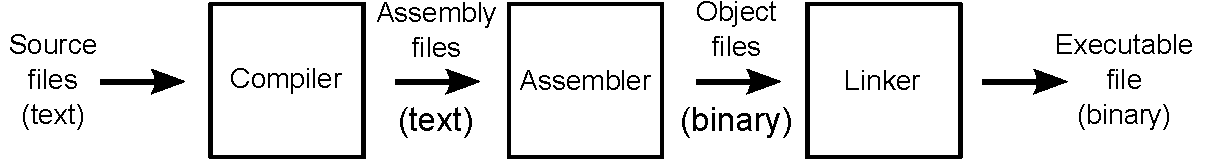
\includegraphics{fig/comp.pdf}}
    \caption{Compilation chain of a C-like language}
    \label{fig_comp}
\end{figure}

A prominent feature when using any kind of obfuscation is that, when applied in a randomized manner, one can generate a number of different versions of the final malware. These versions are referred to as \emph{mutations} and the quality of an obfuscation technique is often measured by the number of possible mutations it allows.

\subsection{Packing, encryption and oligomorphism}
\emph{Packing} is a technique which uses compression algorithms to scramble the content of the binary file\cite{Symatec08}. A decompression procedure is then added to the compressed malware binary so that when the executable is loaded into memory, it will first decompress the malware code and then proceed to execute it. Packing also reduces file size which helps propagation via size-limited channels e.g. email attachments. 

Another common way of obfuscating binary files is through encryption. Similarily to packing, the main malware body is encrypted using a simple cipher and a decryption procedure is added to the result. The encryption key is often carried with the decryption procedure or can be easily computed from data available to the decryption procedure. Most commonly used ciphers include XOR ciphers, RC4 or TEA. 

By using multiple packers or encryption procedures and keys one can obtain a sizeable number of possible mutations. Malware that generates its mutations in this manner is \emph{oligomorphic}. Although the number of possible mutations is high, the decompression and decryption procedures themselves are not mutated. This produces an opportunity for malware analysts to create signatures that target these procedures and detect oligomorphic malware based on them.

\subsection{Polymorphism}
\label{s_polymorph}
The solution to the shortcomings of oligomorphic malware is to mutate their decompression and decryption procedures. \emph{Polymorphic} malware achieves this by applying obfuscations to the code of those procedures. Depending on the obfuscations applied the number of possible mutations rises dramatically. The result is malware whose mutations share almost no resemblance to each other as binary files and thus cannot be generally detected by matching against byte signatures of binary files. A list of commonly used obfuscations follows.

\paragraph*{Dead code insertion}
Code with no effect is inserted into the original code. Common examples include inserting \texttt{NOP} instructions between original assembly instructions or performing \texttt{XOR} operations over two identical operands. While very simple to implement, it is also very simple to reverse the transformation and recover the orignal code. Combined with other obfuscations however, the inserted code may be further transformed and made very hard to recognize as dead.

\begin{figure}[H]
    \centering
    \scalebox{0.65}{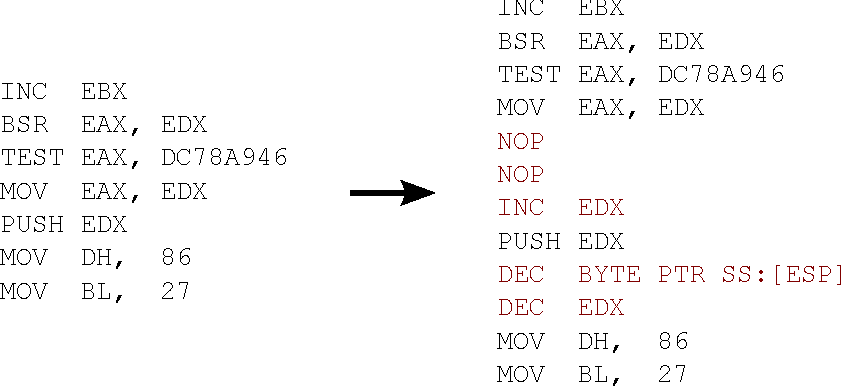
\includegraphics{fig/obf_dci.pdf}}
    \caption{Example of dead code insertion}
    \label{fig_obf_dci}
\end{figure}

\paragraph*{Register reassignment}
Operands of assembly code instructions are often stored in registers. The obfuscation changes the registers in which the operands of instructions are stored. The number of possible mutations this obfuscations allows can be large depending on the instructions used and number of registers available, however it can be easily circumvented via using inexact byte signatures. This technique was prominently used in the Win95/Regswap virus.

\begin{figure}[H]
    \centering
    \scalebox{0.65}{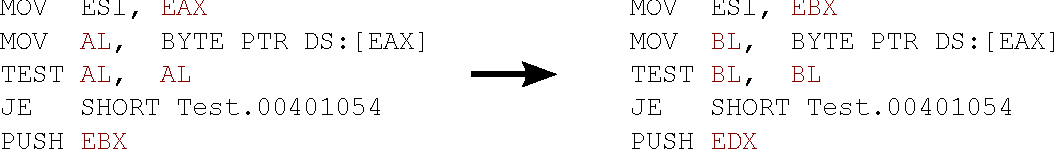
\includegraphics{fig/obf_regswap.pdf}}
    \caption{Example of register reassignment}
    \label{fig_obf_regswap}
\end{figure}

\paragraph*{Subroutine reordering}
Also called code permutation is a transformation where standalone code segments such as subroutines or basic blocks can be randomly reordered to produce up to $N!$ mutations, where $N$ is the number of such segments. W32/Ghost is a common example of a virus that uses this obfuscation.

\begin{figure}[H]
    \centering
    \scalebox{0.65}{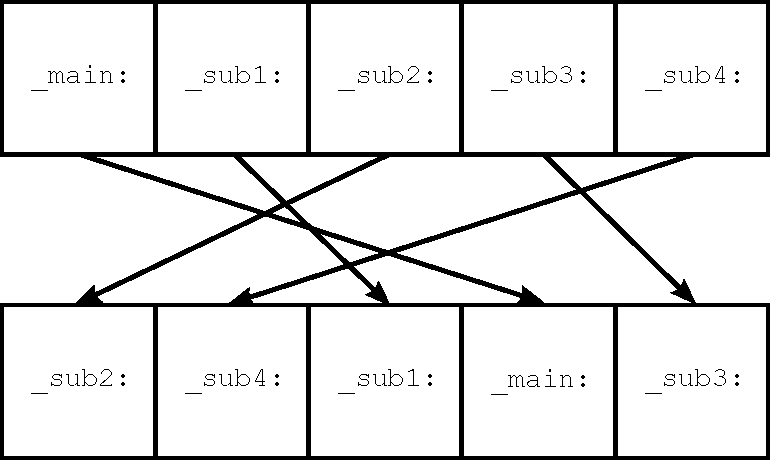
\includegraphics{fig/obf_perm.pdf}}
    \caption{Example of subroutine reordering}
    \label{fig_obf_perm}
\end{figure}

\paragraph*{Instruction substitution}
The effect of a single instruction in code can be often emulated via a sequence of instructions. Typical examples are simple arithmetic and boolean operations which can be emulated in a number of ways each. Other substitutions include moves between registers being replaced by \texttt{PUSH} and \texttt{POP} instructions on the assembly level.

\begin{figure}[H]
    \centering
    \scalebox{0.65}{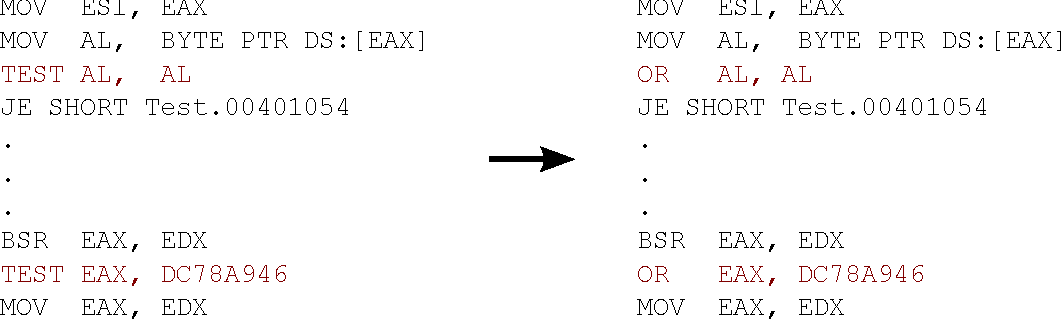
\includegraphics{fig/obf_instrsub.pdf}}
    \caption{Example of instruction substitution}
    \label{fig_obf_instrsub}
\end{figure}

\paragraph*{Code transposition}
Similar to subroutine reodreding, this obfuscation reorders instructions to change the binary file. If the reordered instructions are dependent, original execution order is restored via unconditional jumps. Depending on the code representation, determining whether two instructions are dependent may require a non-trivial analysis.

\begin{figure}[H]
    \centering
    \scalebox{0.65}{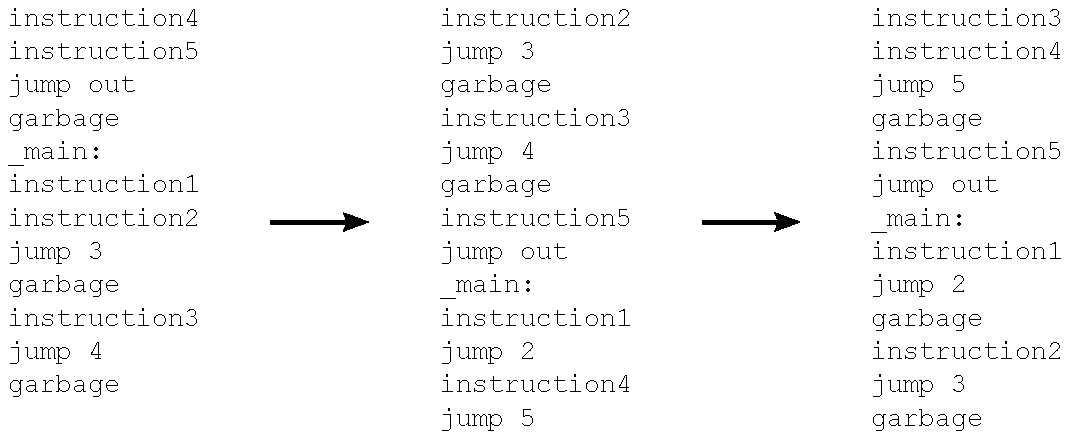
\includegraphics{fig/obf_trans.pdf}}
    \caption{Example of code transposition}
    \label{fig_obf_trans}
\end{figure}

\paragraph*{Code integration}
A technique that uses another executable binary file for obfuscation. The malware excutable targets a host executable, disassembles it, inserts its own code into it and reassembles the host, preserving its original functionality. This way the malware can generate as many mutations as there are executable binaries in the host system, while providing other advantages like obfuscating the malware's entry point, since the execution of malware code is interleaved with the execution of the host binary. This obfuscation was introduced in the famous W95/Zmist virus.

\subsection{Metamorphism}
The main weakness of polymorphic malware was the fact that even though the unpacking and decryption procedures were mutated, the main malicious code was not. By allowing the malware to run in a controlled environment, the malicious code would eventually appear in memory and could be matched against a byte signature.

\emph{Metamorphic} malware answers this weakness by applying obfuscating code transformations to the whole code of the malware, including the malicious parts. This way the malware changes significantly from one mutation to another and leaves little space for simple byte signature detection. The downside to this malware is the complexity of a mutation engine capable of such code transformations. Figure \ref{fig_metamorph} shows the process of generating a new mutation from an old one, once a metamorphic malware is executed. The best example of an implementation is the virus Simile and its MetaPHOR mutation engine.

\begin{figure}[H]
    \centering
    \scalebox{0.65}{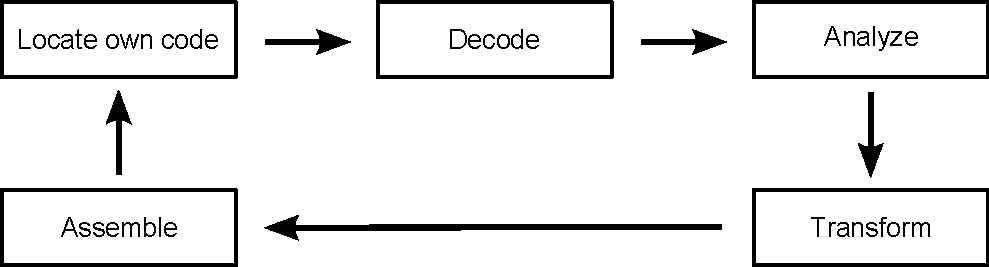
\includegraphics{fig/metamorph.pdf}}
    \caption{Mutation stages of a metamorphic malware}
    \label{fig_metamorph}
\end{figure}

\section{Syntactic Detection}
Historically malware detection techniques were centered around syntactic properties of a binary file under inspection. These methods often look for specific byte sequences in files and any file that contains a byte sequence that is deemed malicious is marked as malware. The detection rates of these methods were heavily dependent on the length of the byte sequence which was looked for and the structure of the malware code. The advantages of this approach, to this day, are speed and scalability. The main disadvantage is that they are easy to bypass using any kind of obfuscation. To circumvent this, several modifications were introduced.

\paragraph*{Wildcards} The modification adds symbols with special semantics into the byte signature. Consider figure \ref{fig_wildcards}. The upper sequence of bytes is a part of the W32/Beast virus and the lower sequence is the wildcard byte signature used to detect it. The \texttt{?} symbol marks an optional occurence of a half-byte, while \texttt{\%2} says that the next byte may occur twice in the following two bytes.

\begin{figure}[H]
    \centering
    \scalebox{0.65}{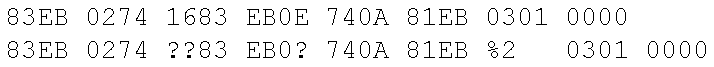
\includegraphics{fig/wildcards.pdf}}
    \caption{An example of a wildcard byte signature}
    \label{fig_wildcards}
\end{figure}

\paragraph*{Mismatches} Allow an inexact matching of a byte signature. The following example illustrates an algorithm that allows a mismatch of three bytes. After encountering a mismatch, the algorithm notes the mismatch and the next byte of the signature is used for matching. Figure \ref{fig_mismatch} shows a byte signature and three malware byte sequences that the signature matches.

\begin{figure}[H]
    \centering
    \scalebox{0.65}{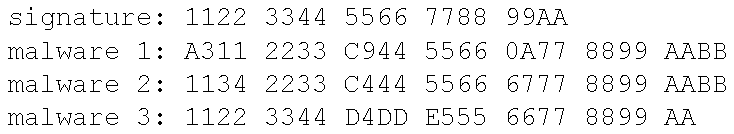
\includegraphics{fig/mismatch.pdf}}
    \caption{An example of mismatch byte signatures}
    \label{fig_mismatch}
\end{figure}

\subsection{Algorithmic Scanning}
As obfuscated malware grew more commonplace, detection moved to methods that used malware-specific heuristics for detection. An example of such a heuristic is \emph{smart scanning} which was able to beat simple obfuscations by ignoring \texttt{NOP} instructions or by performing matching only in the scope of basic blocks. \emph{X-Ray scanning} on the other hand targeted malware encrypted with weak ciphers. The method used a brute-force attack to uncover the encryption key and once uncovered performed a byte signature matching over the decrypted body. \emph{Filtering} restricted detection to only those files that could contain malicious code.

Finally a generalized version of heuristic detection was dubbed \emph{algorithmic scanning} and introduced specialized malware description languages that aided the creation of detection procedures. An algorithmic detector was then essentially an interpreter of such a language coupled with a database of detection procedures.

\subsection{Code Emulation}
Emulation-based detection methods were developed as an answer to strong polymorphic malware. In an emulation-based detector, the suspicious executable is allowed to run in a controlled environment. In case of a polymorphic malware, the packed or encrypted malicious code will eventually be exposed in the memory of the environment, where it can be again detected by a byte signature.

The success of this method is however dependent on how precisely the controlled environment simulates a real host. If the malware detects that its running in a controlled environment it can halt any malicious activity and perform bening computations. Or the malware can exhibit its malicious behavior only under certain conditions, such as time or a certain host system language localization.

The main disadvantage however is that an antivirus must not hinder a legitimate user in his use of a system and its files. Therefore the detection method must be fast, which in the context of an emulation-based detector means that it has only limited time to spend on a single file. So the simplest way for a malware to avoid detection is to perform benign computation until the detector runs out of time.

\section{Behavioral Detection}
\label{s_behav_det}
With the advent of strongly polymorphic and metamorphic malware syntactic detectors proved to be insufficient. The reason for this was the large number of syntactic signatures that detection of such malware would require. Research has even proved that a syntactically undetectable malware is possible\cite{Filiol07}. 

The problem of strongly obfuscated malware was further demonstrated by the outbreak of the Storm worm in 2007. The authors of Storm did not equip the worm with its own mutation engine, instead they released a large number of mutations in bursts into the public internet. This way the antivirus companies were not able to reverse-engineer the worms mutation engine, thus come up with a suitable heuristic detection procedure in time.

The proposed solution to this are behavioral detection methods, which abstract from how the malicious behavior is implemented and aim to detect the malicious behavior itself. Many of the detection methods are directly related to methods used in software testing and quality assurance. The advantage of this approach is its generality and robustness against any kind of syntactic obfuscation. The main disadvantage is the high computational complexity of these methods. 

Figure \ref{fig_gen_behav_detector} shows a schema of a generic behavioral detector. After initial data collection a higher abstraction is built by interpreting the collected data. This abstraction can now be used to enrich the database of malicious behavior signatures if the input is known to be malicious. If the input is not known to be malicious a matching of the abstraction is done against the database. Finally a prediction whether the input is malicious or not is made. If the input is malicious, its behavior abstraction can be used to enrich the database further.

\begin{figure}[H]
    \centering
    \scalebox{0.3}{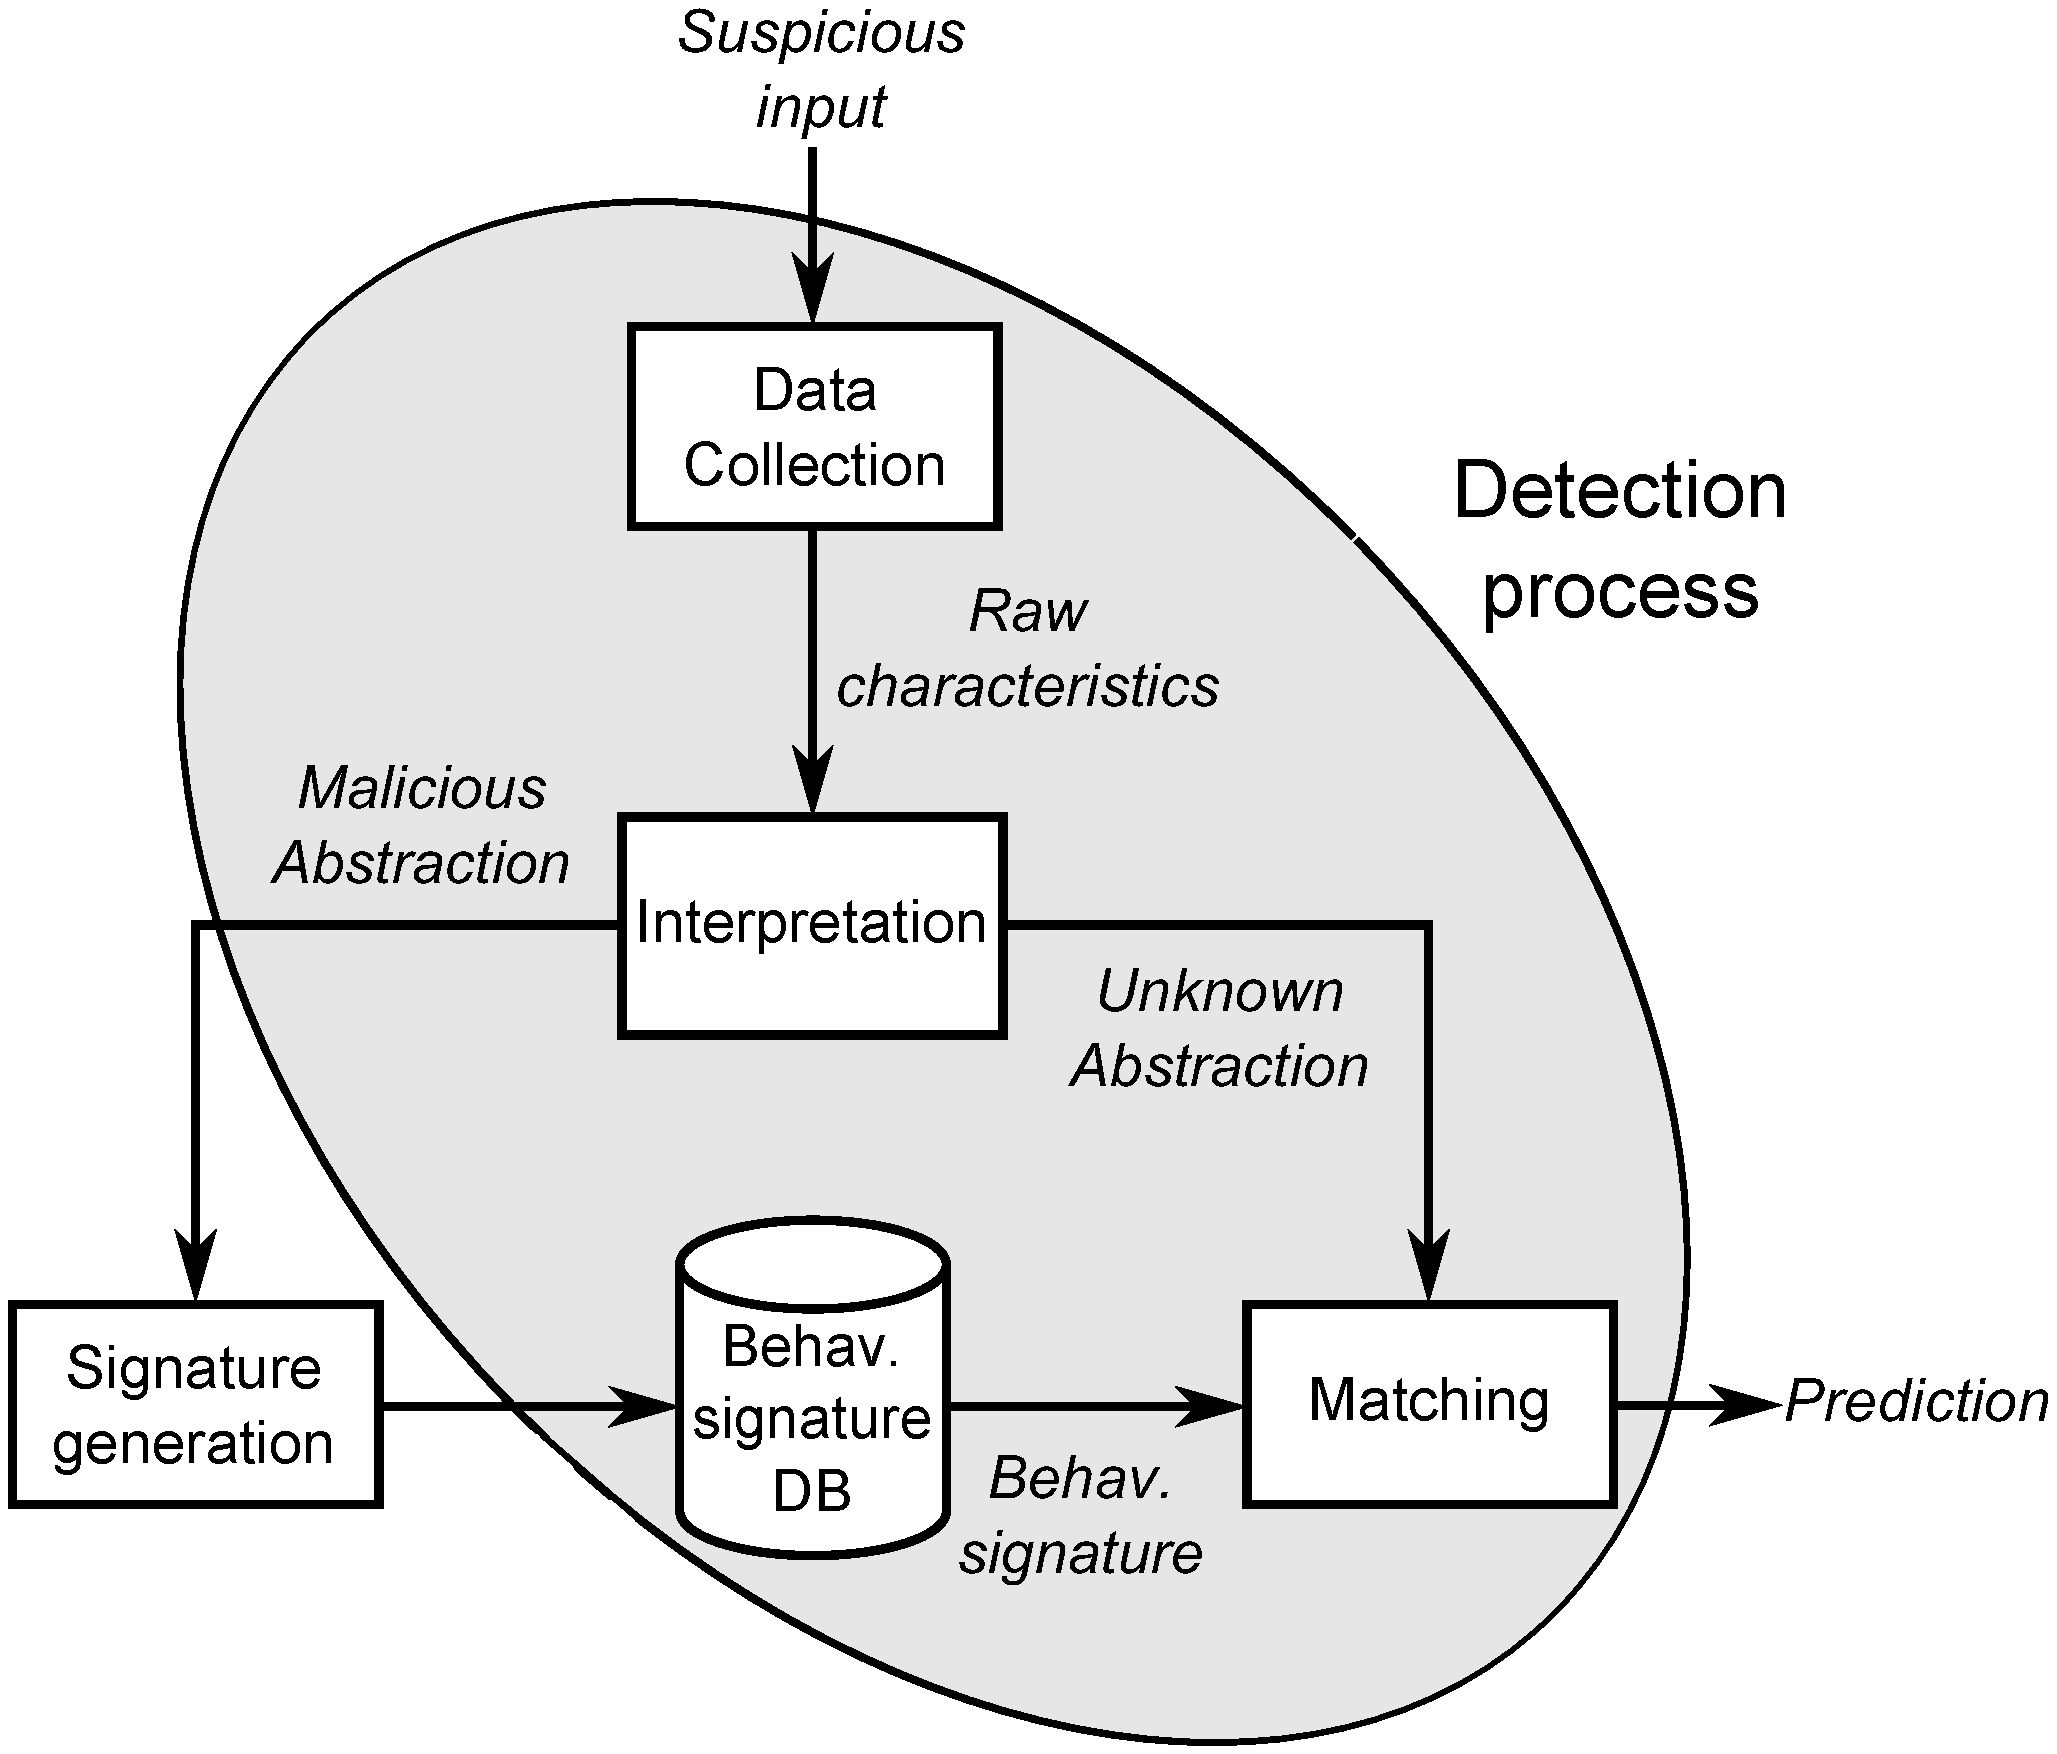
\includegraphics{fig/gen_behav_detector.pdf}}
    \caption{A generalized behavioral detector}
    \label{fig_gen_behav_detector}
\end{figure}

Figure \ref{fig_behav_det_tax} shows a taxonomy of behavioral detectors as presented in \cite{Jacob08}. The diagram is vertically split into two parts according to the general approach to detection. The parts themselves are divided further horizontally to describe the data structures and algorithms used in each of the detection stages introduced in figure \ref{fig_gen_behav_detector}. Finally the lower part of the figure shows how behavioral signatures are generated from known malware, while the upper part shows how behavior is extracted from the environment in which malware can appear.

\subsection{Simulation-based Detection}
Based in black-box testing, this method analyzes malware behavior in a monitored environment during execution. This environment may be controlled, in which case code emulation is employed, or in some applications the malware may be left to run on a live host.

\paragraph*{Data collection} Detectors of this type perform data collection by monitoring events that the malware causes in the host system, be it a controlled environment or a live host. Sequences of these events are called \emph{traces}. An example of a trace is a sequence of system calls or a sequence of sent network packets.

\begin{figure}[H]
    \centering
    \scalebox{0.35}{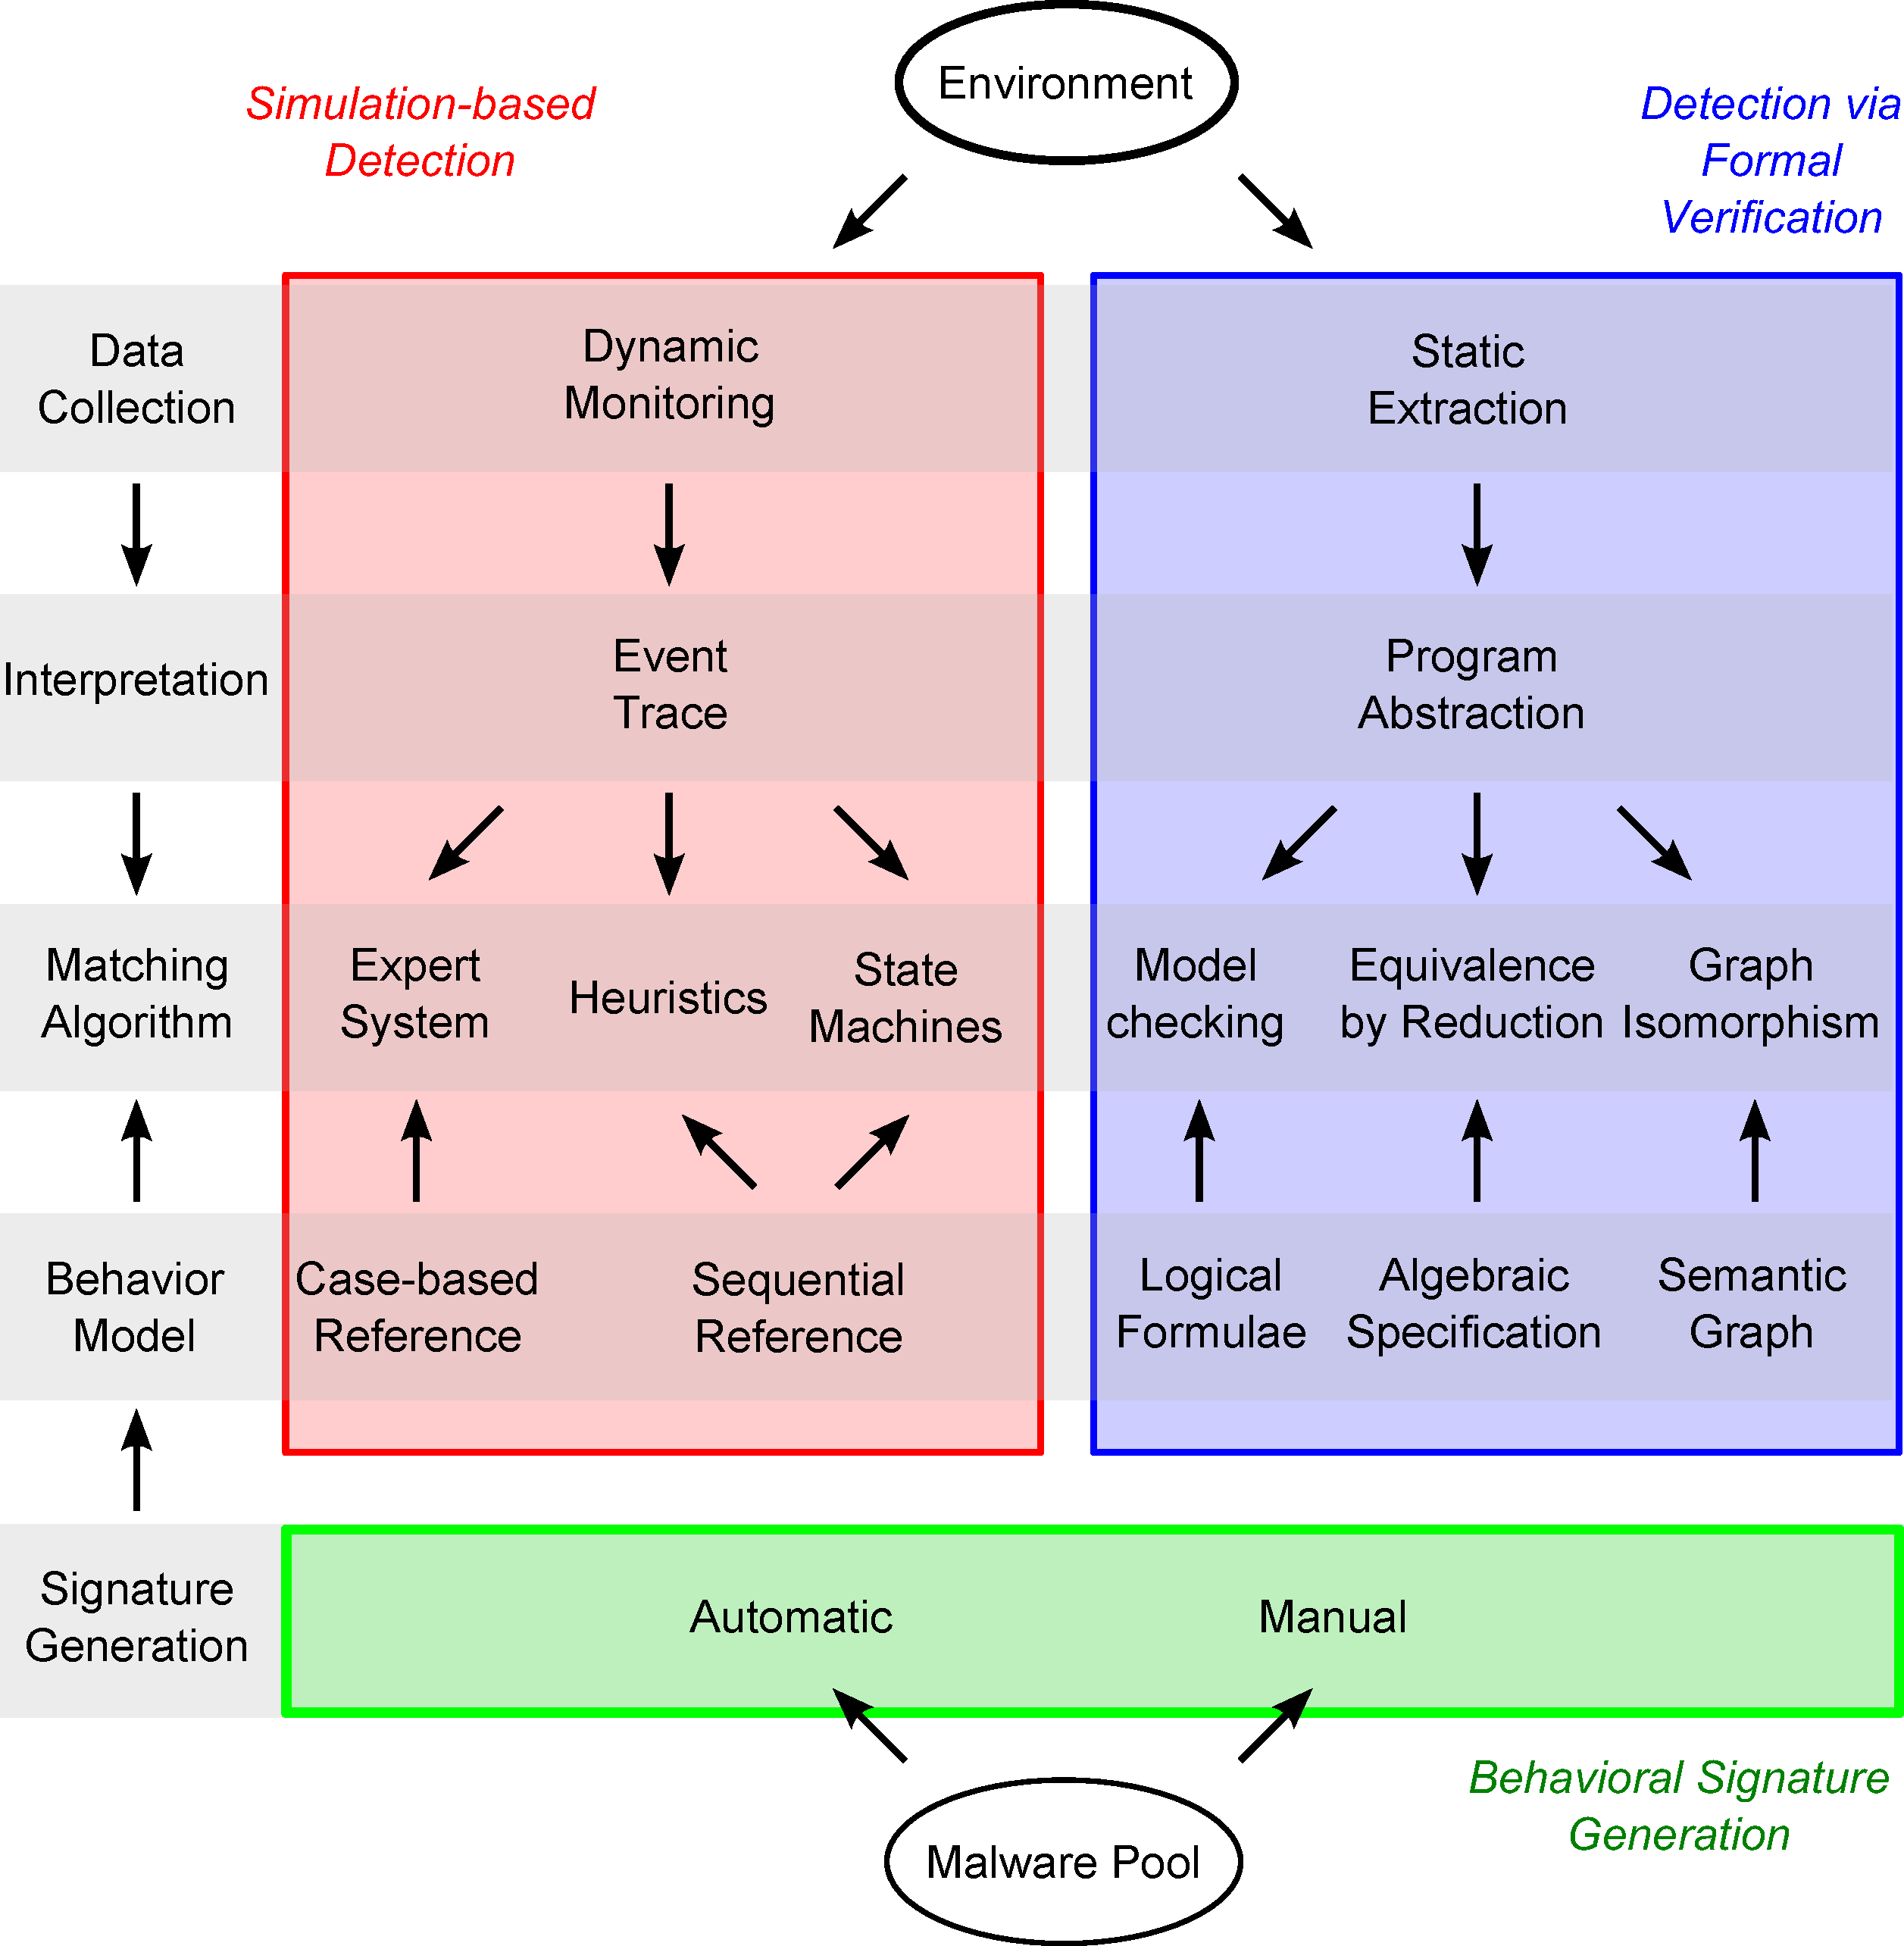
\includegraphics{fig/gen_behav_tax.pdf}}
    \caption{A taxonomy of behavioral detectors}
    \label{fig_behav_det_tax}
\end{figure}

\paragraph*{Interpretation} Traces are then often interpreted into \emph{atomic behaviors}. These often represent a high level event in the host system e.g. opening of a file or establishing a network connection. Atomic behaviors can then be organized into sequences forming a behavioral fingerprint of an inspected process.

\paragraph*{Matching} Matching is performed based on the model of malicious behavior. Common models include weighted rule tables, graphs of atomic behaviors or state machines. The prediction is then made based on a sum of weights and a threshold, existence of a path in a graph or the acceptance of a state machine.

The advantages and disadvantages of this approach are closely tied to its dynamic nature. One can only observe one of many possible behaviors at once, if code emulation is employed, the malware can simply not perform malicious actions in the controlled environment and allowing execution on a live host presents considerable risks.

\subsection{Detection via Formal Verification}
Behavioral detection is commonly associated with dynamic analysis. This may seem short-sighted given that the behavior of a program is fully specified by its code. In the context of information system, formal verification is used to mathematically prove or disprove that the system satisfies a given specification or that the system has a certain property. Applied to malware detection the verified system is a representation of a computer program and the property is the presence of known malicious behavior.

\paragraph*{Data collection} Since binary files are the most common representation of malware data collection is done by static extraction. This task mainly involves disassembling the binary file into assembly code, but unpacking and decryption are often needed as preliminary steps.

\paragraph*{Interpretation} Once a suitable code representation is obtained, methods for formal analysis and verification can be applied to build an abstraction of the program behavior. The abstraction should model the program behavior in such a way that is robust against obfuscations, but on the other hand should also provide a precise enough description so that false positives stay low. Common abstractions include annotated semantic graphs derived from the program data or control flow, expressions in abstract algebras or the state space of the malware.

\paragraph*{Matching} Algorithms used for matching are directly linked to the chosen abstractions and often can be reduced to solving problems tied to the abstraction. In the case of annotated semantic graphs, matching can be reduced to the subgraph isomorphism problem, where malicious behavior signatures are represented as graph fragments and matched. In the case of abstract algebra, the program abstraction is reduced using rewriting rules and checked for equivalence with signatures represented by expressions as well. Finally in the case of a state space abstraction, model checking algorithms are used to investigate whether malicious properties represented by temporal logic formulae are satisfied by the state space.

The main advantage of detection by formal verification is that all possible execution paths, therefore all possible behaviors of a potential malware are analyzed. This means that techniques used to thwart dynamic analysis have little effect. The main disadvantages however are the complexity of static extraction, since binary code is generally difficult to analyze and can be obfuscated easily and the computational complexity of the algorithms used for interpretation and matching. For example general subgraph isomorphism is a NP-complete\cite{Garey79} problem while LTL model checking is a PSPACE-complete problem\cite{Sistla85}.

\chapter{Preliminaries}
\label{ch_prelim}
This chapter introduces theoretical concepts that underlie the methods and algorithms used in the behavioral detector presented in chapter \ref{ch_detector} as well as the {LLVM} compiler infrastructure used to implement it. Abstract interpretation is introduced as a general framework for building static program analyses and tree automata are presented as the formal model used for matching abstracted program behavior with known malicious behavior signatures. The sections on static analysis and abstract interpretation are based on \cite{FAV_Slides16} and corresponding chapters from \cite{Nielson05}. Parts on tree automata and related notions are based on \cite{tata07} and \cite{Babic11}. Finally the overview of the {LLVM} project and its intermediate representation is based on \cite{LLVM14}.

\section{Static Analysis}
The definition of what constitutes a static program analysis varies. Generally the term is used to describe any kind of automated collection of information about a computer program without executing the program. Under this definition, static analyses range from a simple search for syntactic patterns to precise computations over a program abstraction and even model checking which systematically searches the state space of a program.

As a collection of general methods and algorithms, static analysis is traditionally used in compiler optimizations to identify redundant or ineffective code, code generators, where it provides information needed to bridge the gap between code representations and tools for formal verification, where it is used for quality assurance. Recently however information security specialists and malware analysts have also found uses for static analysis when evaluating system vulnerabilities and analyzing malware.

\subsection{Partially Ordered Sets and Lattices}
\begin{defn}[\emph{Partially Ordered Set}]
Let $L$ be a set. A partial ordering $(\sqsubseteq) \; \subseteq L \times L$ is a relation that is \emph{reflexive} ($\forall l \in L: l \sqsubseteq l$), \emph{transitive} ($\forall l_1, l_2, l_3 \in L: l_1 \sqsubseteq l_2 \; \wedge \; l_2 \sqsubseteq l_3 \Rightarrow l_1 \sqsubseteq l_3$) and \emph{anti-symmetric} ($\forall l_1, l_2 \in L: l_1 \sqsubseteq l_2 \; \wedge \; l_2 \sqsubseteq l_1 \Rightarrow l_1 = l_2$). For $(x,y) \in \; \sqsubseteq$ we shall write $x \sqsubseteq y$, and $x \sqsubset y$ if also $x \neq y$. The tuple $(L, \sqsubseteq)$ is called a \emph{partially ordered set}.
\end{defn}

\begin{defn}[\emph{Least Upper Bound}]
Let $(L, \sqsubseteq)$ be a partially ordered set. A subset $Y \subseteq L$ has $l \in L$ as an \emph{upper bound} if $\forall l' \in Y: l' \sqsubseteq l$. An upper bound $l$ of $Y$ is a \emph{least upper bound}, written as $\sqcup Y$, if $\forall l_0 \in L: l \sqsubseteq l_0$, where $l_0$ is an upper bound of $Y$. Symbol $\sqcup$ shall denote the \emph{join} operator and for $\sqcup\{l_1, l_2\}$ we shall write $l_1 \sqcup l_2$.
\end{defn}

\begin{defn}[\emph{Greatest Lower Bound}]
Let $(L, \sqsubseteq)$ be a partially ordered set. A subset $Y \subseteq L$ has $l \in L$ as a \emph{lower bound}, written $\sqcap Y$, if $\forall l' \in Y: l \sqsubseteq l'$. A lower bound $l$ of $Y$ is a \emph{greatest lower bound} if $\forall l_0 \in L: l_0 \sqsubseteq l$, where $l_0$ is a lower bound of $Y$. Symbol $\sqcap$ shall denote the \emph{meet} operator and for $\sqcap\{l_1, l_2\}$ we shall write $l_1 \sqcap l_2$.
\end{defn}

\begin{defn}[\emph{Lattices}]
A \emph{join-semilattice} or \emph{meet-semilattice} is a partially ordered set $(L, \sqsubseteq)$ in which every pair of elements in $L$ has a least upper bound or greatest lower bound, respectively. A semi-lattice is \emph{complete} if every subset of $L$ has a least upper bound or greatest lower bound. Furthemore $\bot = \sqcup \emptyset = \sqcap L$ is the \emph{least element} and $\top = \sqcap \emptyset = \sqcup L$ is the \emph{greatest element}. A \emph{lattice} $(L, \sqsubseteq, \sqcup, \sqcap, \bot, \top)$ is a partially ordered set that is a meet-semilattice and a join-semilattice. A lattice is complete if it is a complete join-semilattice and a complete meet-semilattice.
\end{defn}

\begin{figure}[H]
    \centering
    \scalebox{0.65}{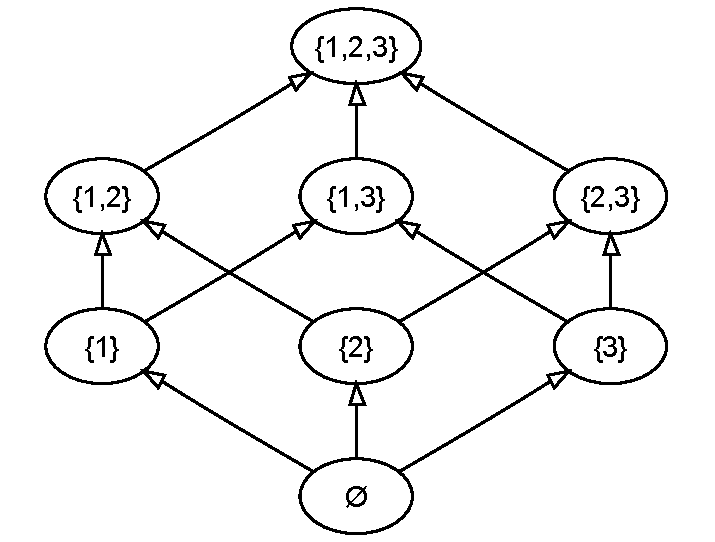
\includegraphics{fig/hasse_diag.pdf}}
    \caption{A Hasse diagram of the $(2^{\{1,2,3\}}, \subseteq, \cup, \cap, \emptyset, \{1,2,3\})$ lattice}
    \label{fig_hasse_diag}
\end{figure}

\begin{defn}[\emph{Chain}]
Let $(L, \sqsubseteq)$ be a partially ordered set. A \emph{chain} from $x_0$ to $x_n$ is a set $C = \{x_0, x_1, \dots, x_n\} \subseteq L$ where $x_0 \sqsubset x_1 \sqsubset x_2 \sqsubset \dots \sqsubset x_n$. 
\end{defn}

\begin{defn}[\emph{$\sqcup-$continuous function}]
Let $(A, \sqsubseteq_A)$ and $(B, \sqsubseteq_B)$ be lattices and $f: A \rightarrow B$ a function. Function $f$ is \emph{monotone} if $\forall x, y \in L: x \sqsubseteq_A y \Rightarrow f(x) \sqsubseteq_B f(y)$. Furthermore $f$ is \emph{$\sqcup-$continuous} if $f(\sqcup C) = \sqcup\{f(c) | c \in C\}$ for every chain $C \subseteq A$.
\end{defn}

\begin{defn}[\emph{Least Fixed Point}]
Let $(L, \sqsubseteq)$ be a lattice and $f: L \rightarrow L$ a function. An element $x \in L$ is a \emph{fixed point} of $f$ if $f(x) = x$ and a \emph{least fixed point} if $\forall y \in L: f(y) = y \Rightarrow x \sqsubseteq y$.
\end{defn}

\begin{thm}[\emph{Kleene Fixed Point}]
Let $(L, \sqsubseteq, \sqcup, \sqcap, \bot, \top)$ be a lattice and $f: A \rightarrow A$ a $\sqcup-$continuous function. The least fixed point of $f$ is $\mu f = \sqcup\{f^i(\bot)|i \geq 0\}$.
\end{thm}

The Kleene fixed point theorem essentially tells that by repeatedly applying a $\sqcup-$ continuous function $f$ over a lattice starting from the least element of the lattice, one will eventually reach the least fixed point of $f$ while forming a chain along the way. This is very useful when designing iterative algorithms over data that form a lattice. Such an algorithm iteratively refines an approximate solution and is guaranteed to terminate if the lattice is finite and the algorithm has the properties of a $\sqcup-$continuous function.

\subsection{Abstract Interpretation}
Pioneered by Patrick and Radhia Cousot in \cite{Cousot77}, \emph{abstract interpretation} is a framework for building static analyses based on lattices. The basic idea is to model the states a computer program can be in via \emph{abstract contexts} over an \emph{abstract domain} that is suitable for gathering the information that we want from the static analysis. If we wish to know the possible values of integer variables in a program, we may use intervals of natural numbers or convex polyhedra as our abstract domain. If we're collecting information about strings, we will probably use an abstract domain based in formal language theory.

Each instruction in the program is assigned an \emph{abstract transformer} which emulates the execution of the instruction in the abstract domain. An addition over two integer variables will modify the intervals corresponding to those variables in the abstract context of the program. Finally the analysis is done by iteratively computing the abstract contexts of the program until the computation reaches a fixed point. In some cases however, e.g. programs with loops, the reaching of a fixed point is not guaranteed. A \emph{widening} operator over abstract contexts which over-approximates the precise iterative solution may be introduced to guarantee termination and speed up the analysis. The application of widening however degrades the results of the analysis. \emph{Narrowing} operators can be applied to the results of a widening to refine the final result of the analysis.

\begin{defn}[\emph{Abstract Interpretation}]
An \emph{abstract interpretation} $I$ of a program $P$ with the instruction set \texttt{Instr} is a tuple $$I = (Q, \circ, \sqsubseteq, \bot, \top, \tau)$$ where
\begin{itemize}
    \item $Q$ is the abstract domain (a set of abstract contexts),
    \item $\circ: Q \times Q \rightarrow Q$ is the \emph{join operator} for accumulation of abstract contexts and $(Q, \circ, \top)$ is a complete join-semilattice,
    \item $(\sqsubseteq) \subseteq Q \times Q$ is a partial ordering defined as $\forall x, y \in Q: x \sqsubseteq y \Leftrightarrow x \circ y = y$ in $(Q,\circ, \top)$,
    \item $\bot$ is the least element of $Q$,
    \item $\top$ is the greatest element of $Q$,
    \item $\tau: \text{\texttt{Instr}}\times Q \rightarrow Q$ defines an interpretation of abstract transformers.
\end{itemize}
\end{defn}

\begin{defn}[\emph{Widening}]
Let $I = (Q, \circ, \sqsubseteq, \bot, \top, \tau)$ be an abstract interpretation. For the binary \emph{widening} operator $\triangledown$ the following holds:
\begin{itemize}
    \item $\triangledown: Q \times Q \rightarrow Q$,
    \item $\forall C,D \in Q: (C \circ D) \sqsubseteq (C \triangledown D)$,
    \item for all infinite sequences $(C_0, C_1, \dots, C_n, \dots) \in Q^\omega$, it holds that the infinite sequence $(s_0, s_1, \dots, s_n, \dots)$ defined recursively as $s_0 = C_0, \; s_n = s_{n-1} \triangledown C_n$ is not strictly increasing.
\end{itemize}
\end{defn}

\begin{defn}[\emph{Narrowing}]
Let $I = (Q, \circ, \sqsubseteq, \bot, \top, \tau)$ be an abstract interpretation. For the binary \emph{narrowing} operator $\triangle$ the following holds:
\begin{itemize}
    \item $\triangle: Q \times Q \rightarrow Q$,
    \item $\forall C,D \in Q: D \sqsubseteq C \Rightarrow (D \sqsubseteq (C \triangle D) \sqsubseteq C)$,
    \item for all infinite sequences $(C_0, C_1, \dots, C_n, \dots) \in Q^\omega$, it holds that the infinite sequence $(s_0, s_1, \dots, s_n, \dots)$ defined recursively as $s_0 = C_0, \; s_n = s_{n-1} \triangle C_n$ is not strictly decreasing.
\end{itemize}
\end{defn}

To ensure certain properties of the abstract interpretation with regard to the analyzed program, one may employ \emph{Galois connections}. The most common property investigated is \emph{soundness} which ensures that the abstraction over-approximates the behavior of the analyzed program and thus can only produce false positives. In the context of malware detection, this means that it may find malicious behavior that is present in the abstract domain, but not in the program itself, assuming a precise specification of what malicious behavior is given.

\section{Tree Automata}
Introduced as a generalization of word languages in formal language theory, tree languages describe sets of directed trees or \emph{terms}. Their defining formalisms \emph{tree automata} and \emph{regular tree grammars} found a wide array of uses. Automata in areas of formal verification and automated reasoning as parts of decision procedures for logics. Grammars in areas of computational linguistics and programming languages.

\subsection{Ranked Alphabets, Terms and Trees}
\begin{defn}[\emph{Ranked Alphabet}]
Let $\mathcal{F}$ be a finite set of symbols, $\mathbb{N}$ the set of natural numbers and $Arity: \mathcal{F} \rightarrow \mathbb{N}$ a function. A \emph{ranked alphabet} is the tuple $(\mathcal{F}, Arity)$. The \emph{arity} of a symbol $f \in \mathcal{F}$ is denoted $Arity(f)$ and the set $\mathcal{F}_p = \{f \; | \; f \in F \wedge Arity(f) = p\}$ is the set of symbols of arity $p$. Symbols of arity $0, 1, \dots, p$ are respectively called constants, unary symbols, \dots, $p$-ary symbols.
\end{defn}

\begin{defn}[\emph{Terms}]
Let $\mathcal{F}$ be a ranked alphabet and $\mathcal{X}$ a set of constants called \emph{variables}. We assume that $\mathcal{F}_0 \cap \mathcal{X} = \emptyset$. The set $T(\mathcal{F}, \mathcal{X})$ of \emph{terms} over the ranked alphabet $\mathcal{F}$ and variables $\mathcal{X}$ is the smallest set defined by:
\begin{itemize}
    \item $\mathcal{F}_0 \subseteq T(\mathcal{F}, \mathcal{X})$,
    \item $\mathcal{X} \subseteq T(\mathcal{F}, \mathcal{X})$,
    \item if $p \geq 1, \; f \in \mathcal{F}_p, \; t_1,\dots, t_p \in T(\mathcal{F}, \mathcal{X})$, then $f(t_1,\dots, t_p) \in T(\mathcal{F}, \mathcal{X})$.
\end{itemize}
If $\mathcal{X} = \emptyset$ then $T(\mathcal{F}, \mathcal{X})$ is also written as $T(\mathcal{F})$. A term $t \in T(\mathcal{F})$ is called a \emph{ground term}. A term $t \in T(\mathcal{F}, \mathcal{X})$ is \emph{linear} if each variable occurs at most once in $t$.
\end{defn}

\begin{defn}[\emph{Tree Domain}]
Let $\mathbb{N}$ be the set of natural numbers and $\mathbb{N}^*$ the \emph{free monoid}\footnote{for a definition see \cite{Lothaire83}} generated by $\mathbb{N}$ with concatenation $(\cdot)$ as the operation and the empty string $\varepsilon$ as the identity. The \emph{prefix order} $(\leq) \subseteq \mathbb{N}^* \times \mathbb{N}^*$ is defined as: $u \leq v \overset{\text{def}}{\Longleftrightarrow} \exists w \in \mathbb{N}^*: v = u \cdot w$. For $u \in \mathbb{N}^*$ and $n \in \mathbb{N}$, the \emph{length} $|u|$ is defined inductively: $|\varepsilon| = 0, \; |u \cdot n| = |u| + 1$. A set $S$ is \emph{prefix-closed} if $u \leq v \wedge v \in S \Rightarrow u \in S$. A \emph{tree domain} is a finite non-empty prefix-closed set $D \subset \mathbb{N}^*$ satisfying the following property: $u \cdot n \in D \Rightarrow \forall 1 \leq j \leq n: u \cdot j \in D$.
\end{defn}

\begin{defn}[\emph{Finite Ordered Tree}]
Let $T(\mathcal{F}, \mathcal{X})$ be a set of terms and $D$ a tree domain. A term $t \in T(\mathcal{F}, \mathcal{X})$ can be represented as a \emph{finite ordered tree} which is a mapping $t: D \rightarrow \mathcal{F} \cup \mathcal{X}$ satisfying the following:
\begin{itemize}
    \item $\forall u \in D:$ if $t(u) \in \mathcal{F}_n, \; n \geq 1$ then $\{j \; | \; u \cdot j \in D\} = \{1, \dots, n\}$
    \item $\forall u \in D:$ if $t(u) \in \mathcal{F}_0$ then $\{j \; | \; u \cdot j \in D\} = \emptyset$
\end{itemize}
The domain of tree $t$ shall be written as $dom(t)$ and each element in $dom(t)$ represents a \emph{position} in $t$. The symbol $t(\varepsilon)$ is called the \emph{root symbol} of $t$.
\end{defn}

\begin{defn}[\emph{Height}]
Let $t \in T(\mathcal{F}, \mathcal{X})$ be a term. The \emph{height} of the term $t$, denoted $height(t)$ is defined inductively as
\begin{equation*}
    height(t) = 
    \begin{cases}
        0 & \text{ if } t \in \mathcal{X}\\
        1 & \text{ if } t \in \mathcal{F}_0\\
        1 + max(\{height(t_i) \; | \; i \in \{1, \dots, n\}\}) & \text{ if } t(\varepsilon) \in \mathcal{F}_n
    \end{cases}
\end{equation*}
\end{defn}

\begin{figure}[H]
    \centering
    \scalebox{0.7}{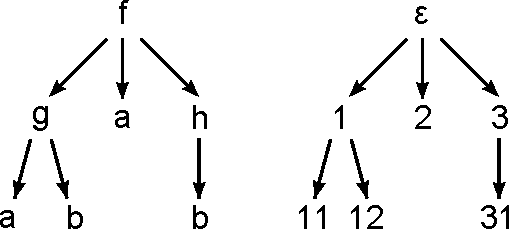
\includegraphics{fig/tree_domain.pdf}}
    \caption{An example of a tree $t$ (left) and its tree domain $D$ (right). $height(t) = 3$}
    \label{fig_tree_domain}
\end{figure}

\begin{defn}[\emph{Subterm}]
Let $t \in T(\mathcal{F}, \mathcal{X})$ be a term. A \emph{subterm} of $t$ at position $p$ denoted $t|_p$ is defined by the following:
\begin{itemize}
    \item $dom(t|_p) = \{j \; | \; pj \in dom(t)\}$,
    \item $\forall q \in dom(t|_p): t|_p(q) = t(pq)$.
\end{itemize}
\end{defn}

\begin{defn}[\emph{Substitution}]
A \emph{substitution} is a mapping $\sigma: \mathcal{X} \rightarrow T(\mathcal{F}, \mathcal{X})$ such that the domain of $\sigma$ is a subset of variables $x \in \mathcal{X}$ and $\sigma(x) \neq x$. The substitution $\{x_1 \leftarrow t_1, \dots, x_n \leftarrow t_n\}$ is an identity on $\mathcal{X} \setminus \{x_1, \dots, x_n\}$ and maps $x_i \in \mathcal{X}$ on $t_i \in T(\mathcal{F}, \mathcal{X})$, for $1 \leq i \leq n$. A \emph{ground substitution} is a substitution into $T(\mathcal{F})$, meaning that all variables in a term $t \in T(\mathcal{F}, \mathcal{X})$ are substituted. Substitutions can be extended to $T(\mathcal{F}, \mathcal{X})$ in the following manner: $$\forall f \in \mathcal{F}_n, \; \forall t_1, \dots, t_n \in T(\mathcal{F}, \mathcal{X}): \sigma(f(t_1, \dots, t_n)) = f(\sigma(t_1), \dots, \sigma(t_n)).$$
\end{defn}

\begin{figure}[H]
    \centering
    \scalebox{0.7}{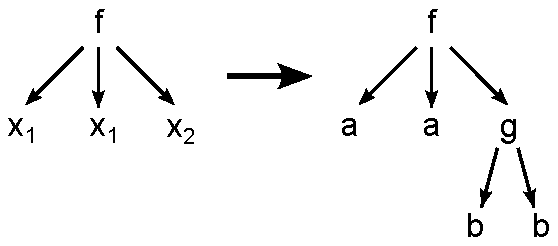
\includegraphics{fig/tree_sub.pdf}}
    \caption{An example of a substitution $\sigma = \{x_1 \leftarrow a, x_2 \leftarrow g(b,b)\}$ to a term $t = f(x_1, x_2, x_2)$}
    \label{fig_tree_sub}
\end{figure}

\begin{defn}[\emph{Context}]
Let $\mathcal{X}_n$ be a set of variables. A linear term $C \in T(\mathcal{F}, \mathcal{X}_n)$ is called a \emph{context} and the expression $C[t_1,\dots,t_n]$ denotes the term $C\{x_1 \leftarrow t_1, \dots, x_n \leftarrow t_n\}$ for $t_1, \dots, t_n \in T(\mathcal{F})$. We denote by $\mathcal{C}^n(\mathcal{F})$ the set of contexts over $(x_1, \dots, x_n)$. As a special case we denote by $\mathcal{C}(\mathcal{F})$ the set of contexts over a single variable. A context is \emph{trivial} if it is reduced to a single variable. Given a context $C \in \mathcal{C}(\mathcal{F})$, we denote by $C^0$ the trivial context, $C^1$ is equal to $C$ and $C^n = C^{n-1}[C]$ is a context in $\mathcal{C}(\mathcal{F})$.
\end{defn}

\subsection{Finite Tree Automata}
An extension of finite automata which work on words, finite tree automata deal with finite ordered ranked trees --- meaning the trees are over a ranked alphabet, or finite ordered trees with bounded rank --- meaning that the trees can be encoded as finite ordered ranked trees. Indeed words over a finite alphabet can be viewed as terms over a ranked alphabet of unary symbols and a constant acting as a terminator. For example the word $xyz$ over the alphabet $\Sigma = \{x,y,z\}$ ca be viewed as the term $t = x(y(z(\#)))$ over the ranked alphabet $\mathcal{F} = \{x(), y(), z(), \#\}$ where $\#$ is the added constant.

Similarly to finite automata, finite tree automata can be deterministic and nondeterministic. Finite tree automata however have different properties depending on how the computation of the automaton is performed. When the computation starts from the leaves of the tree working its way to the root, the automaton is referred to as \emph{bottom-up}. In the opposite case the automaton is a \emph{top-down} one.

Depending on the direction of computation, determinism has different consequences on the expressive power of the automaton. Determnistic bottom-up finite tree automata have the same power as nondeterministic ones and nondeterministic top-down ones. However deterministic top-down finite tree automata are less powerful \cite{tata07}. This work will only consider finite bottom-up tree automata onwards, referring to them as FTA.

\begin{defn}[\emph{Finite Bottom-Up Tree Automaton}]
A \emph{nondeterministic} FTA over a ranked alphabet $\mathcal{F}$ is a tuple $$\mathcal{A} = (Q, \mathcal{F}, Q_f, \Delta)$$ where
\begin{itemize}
    \item $Q$ is the set of (unary) states
    \item $Q_f \subseteq Q$ is the set of final states
    \item $\Delta$ is the set of transition rules of the form $f(q_1(x_1), \dots, q_n(x_n)) \rightarrow q(f(x_1, \dots, x_n))$, where $n \geq 0$, $f \in \mathcal{F}$, $q_1, \dots, q_n \in Q$, $x_1, \dots, x_n \in \mathcal{X}$.
\end{itemize}
A FTA is \emph{deterministic} if no two rules in $\Delta$ have the same left-hand side.
\end{defn}

\begin{defn}[\emph{Move Relation}]
Let $\mathcal{A} = (Q, \mathcal{F}, Q_f, \Delta)$ be a NFTA over $\mathcal{F}$. The \emph{move relation} $\rightarrow_{\mathcal{A}}$ between terms $t,t' \in T(\mathcal{F} \cup Q)$ is defined by
\begin{equation*}
    t \rightarrow_{\mathcal{A}} t' \Leftrightarrow
    \begin{cases}
        \exists C \in \mathcal{C}(\mathcal{F} \cup Q), \exists u_1, \dots, u_n \in T(\mathcal{F}),\\
        \exists f(q_1(x_1), \dots, q_n(x_n)) \rightarrow q(f(x_1, \dots, x_n)) \in \Delta,\\
        t = C[f(q_1(u_1), \dots, q_n(u_n))],\\
        t = C[q(f(u_1, \dots, u_n))].
    \end{cases}
\end{equation*}
By $\rightarrow_{\mathcal{A}}^{*}$ we denote the transitive and reflective closure of $\rightarrow_{\mathcal{A}}$.
\end{defn}

\begin{defn}[\emph{Recognizable Tree Language}]
A ground term $t \in T(\mathcal{F})$ is \emph{accepted} by a FTA $\mathcal{A} = (Q, \mathcal{F}, Q_f, \Delta)$ if $$t \rightarrow_{\mathcal{A}}^{*} q(t)$$ for some $q \in Q_f$. The set of all ground terms accepted by $\mathcal{A}$, written as $L(\mathcal{A})$, is called the tree language \emph{recognized} by $\mathcal{A}$. A tree language $L$ is \emph{recognizable} if there is a FTA $\mathcal{A}$ for which $L(\mathcal{A}) = L$.
\end{defn}

Consider a NFTA $\mathcal{A} = (Q, \mathcal{F}, Q_f, \Delta)$ where $Q = \{q_a, q_g, q_f\}$, $\mathcal{F} = \{f(,), g(), a\}$, $Q_f = \{q_f\}$ and $\Delta = \{a \rightarrow q_a(a), \; g(q_a(x)) \rightarrow q_g(g(x)), \; f(q_g(x), q_g(y)) \rightarrow q_f(f(x,y))\}$. Figure \ref{fig_ta_run} shows an accepting run of $\mathcal{A}$ on the term $t = f(g(a), g(a))$.

\begin{figure}[H]
    \centering
    \scalebox{0.6}{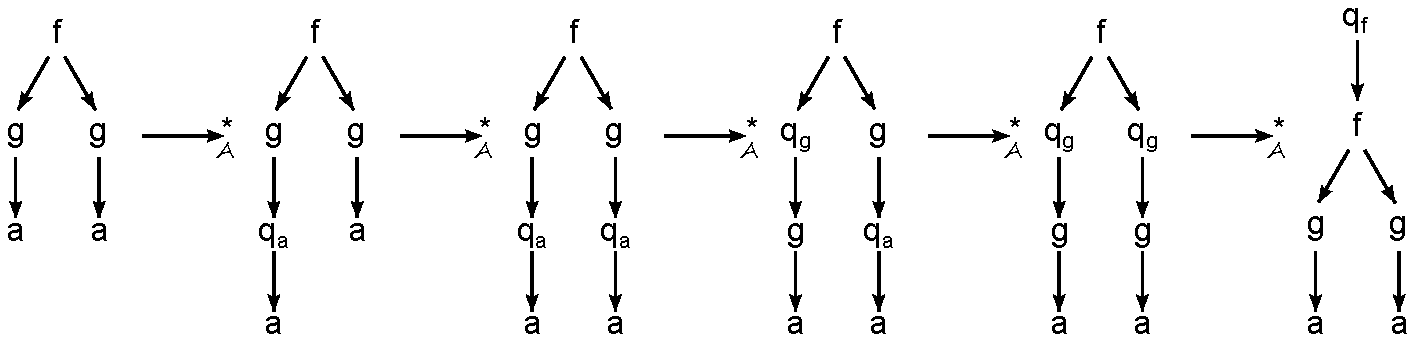
\includegraphics{fig/ta_run.pdf}}
    \caption{An example of an accepting run of a FTA}
    \label{fig_ta_run}
\end{figure}

\subsection{Tree Automata Inference}
The field of \emph{grammatical inference} studies methods and algorithms for machine learning of formal languages by inferring their models from a set of samples. The set of samples may be positive or negative. Positive samples are elements of the inferred language, while negative are not. Research tells that regular word languages cannot be inferred from positive samples only\cite{Gold78}.

The solution is either to learn from positive and negative samples or restricting the inference to less expressive languages. For regular word languages, inferring a minimal finite automaton from positive and negative samples is NP-complete\cite{Gold78}. Inferring a non-minimal automaton is also an option, but there is a risk of exponential blowup of the automaton size. Using less expressive language families on the other hand presents the possibility of inferring a state-minimal automaton from positive samples only\cite{Garcia90}. 

\emph{K-testable languages} present a subclass of regular languages for which the membership of a string can be decided based on the membership of substrings of a bounded length. This section presents \emph{k-testable tree languages} and the construction of a minimal tree automaton from positive samples only.

\begin{defn}[\emph{Placeholders}]
Let $\mathcal{F}$ be a ranked alphabet and $\Xi = \{\xi_f \; | \; f \in \bigcup_{i>0} \mathcal{F}_i\}$ be a new set of variables called \emph{placeholders} such that $\Xi \cap \mathcal{F} = \emptyset$. A variable $\xi_f \in \Xi$ can only be substituted with a tree $t$ for which $t(\varepsilon) = f$. Let $T(\mathcal{F}, \Xi)$ denote the set of trees over the ranked alphabet and placeholders.
\end{defn}

\begin{defn}[\emph{Link}]
Let $t, t' \in T(\mathcal{F}, \Xi)$ be trees. The link operation $t\#t'$ is defined as
\begin{equation*}
    (t\#t')(n) = 
    \begin{cases}
        t(n) & \text{ if } t(n) \notin \Xi \vee (t(n) = \xi_f \wedge f = t'(\varepsilon))\\
        t'(z) & \text{ if } n = y \cdot z, \; t(y) = \xi_{t'(\varepsilon)}, \; y \in dom(y), \; z \in dom(t')
    \end{cases}
\end{equation*}
\end{defn}

\begin{defn}[\emph{Tree Quotient}]
Let $t, t' \in T(\mathcal{F})$ be trees. The \emph{tree quotient} $t^{-1}t'$ is defined as $$t^{-1}t' = \{t'' \in T(\mathcal{F}, \Xi) \; | \; t' = t'' \# t\}$$
\end{defn}

\begin{defn}[\emph{K-Root}]
Let $t \in T(\mathcal{F})$ be a tree. For $k \geq 0$ a \emph{k-root} of $t$ is defined as:
\begin{equation*}
    root_k(t) = 
    \begin{cases}
        t & \text{ if } t(\varepsilon) \in \mathcal{F}_0\\
        \xi_f & \text{ if } f = t(\varepsilon), \; f \in \bigcup_{i > 0}\mathcal{F}_i, \; k = 0\\
        f(root_{k-1}(t_1), \dots, root_{k-1}(t_n)) & \text{ if } t = f(t_1, \dots, t_n), \; height(t) > k > 0
    \end{cases}
\end{equation*}
\end{defn}

\begin{thm}[\emph{K-Testable Tree Language}\cite{Lopez04}]
Let $L \subseteq T(\mathcal{F})$ be a tree language. $L$ is $k$-testable in the strict sense if and only if for any $t_1, t_2 \in T(\mathcal{F})$ such that $root_k(t_1) = root_k(t_2)$, when $t_1^{-1}L \neq 0 \wedge t_2^{-1}L \neq 0$ then it follows that $t_1^{-1}L = t_2^{-1}L$.
\end{thm}

\begin{defn}[\emph{Root Equivalence}]
Trees $t_1, t_2 \in T(\mathcal{F})$ are \emph{root-equivalent with degree k} for some $k \geq 0$, denoted $t_1 ~_k t_2$ if and only if $root_k(t_1) = root_k(t_2)$. The $\sim_k$ relation is also a congruence of finite index.
\end{defn}

\begin{defn}[\emph{$\sim_k$-induced Tree Automaton}]
Let $T' \subseteq T(\mathcal{F})$ be finite set of finite trees. The $A^{\sim_k}(T') = (Q, \mathcal{F}, Q_f, \Delta_0 \cup \Delta_n)$ automaton induced by the root equivalence relation $\sim_k$ is defined as:
\begin{gather*}
    Q = \{root_k(t') \; | \; \exists t \in T': \exists u \in dom(T'): t'|_u\}\\
    Q_f = \{root_k(t) \; | \; t \in T'\}\\
    \Delta_0 = \{f \rightarrow f(f) \; | \; f \in \mathcal{F}_0\}\\
    \Delta_n = \{f(root_k(t_1)(t_1), \dots, root_k(t_n)(t_n)) \rightarrow root_k(f)(f(t_1, \dots, t_n))\ \; | \; n \geq 1, \; f \in \mathcal{F}_n\}
\end{gather*}
\end{defn}

\begin{thm}[\cite{Babic11}]
$L(A^{\sim_k})$ is $k$-testable in the strict sense.
\end{thm}

\begin{thm}[\cite{Garcia93}]
$L(A^{\sim_{k+1}}) \subseteq L(A^{\sim_k})$
\end{thm}

\section{The {LLVM} Compiler Infrastructure}
{LLVM} is a collection of tools and libraries for building compilers, toolchain technologies and code analyzers. At the core of the framework is the {LLVM} intermediate representation (IR). {LLVM IR} is a SSA-based, RISC-like assembly language used to represent code throughout the framework. The IR code can be serialized into a textual or binary form, which allows for compile-time, link-time and even "idle-time" transformations. The core {LLVM} tools are built around the IR and manipulate it. The tools include an assembler to the binary format of the IR, disassembler to the textual form of the IR, an optimizer that runs transformation passes over the IR, a linker which combines serialized IR files and several others.

A number of projects have been made using the {LLVM} framework. The original project is Clang, a compiler front-end for C-like programming languages. However thanks to its language-agnostic nature, front ends for other static and dynamic languages have been made as well as implementations of runtime environments like the Java Virtual Machine.

Another group of projects are static and dynamic code analyzers. Clang includes its own built-in static analyzer which aims to highlight common mistakes and inefficiencies a programmer can make. Another static analyzer is {KLEE}, which uses symbolic execution, a form of abstract interpretation, to generate test cases for code represented in {LLVM IR}. The last example of a static analyzer built on {LLVM} is {LLBMC}, a bounded model checker. As for dynamic analysis, {LLVM} includes several code instrumentation tools, called "sanitizers", which generate additional code for runtime analysis.

\subsection{Intermediate Representation}
The {LLVM IR} is a target-independent, typed assembly language. The code represented in the IR is in the \emph{single static assignment} form which means that each variable in the IR is only assigned once. This means that each use of a variable can be easily traced back to its definition, which immensely simplifies analysis and transformations of the IR. The number of variables that can be assigned this way is not limited. Figure \ref{fig_llvmir} shows a piece of C code and the corresponding {LLVM IR}.

\begin{figure}[H]
    \centering
    \scalebox{0.65}{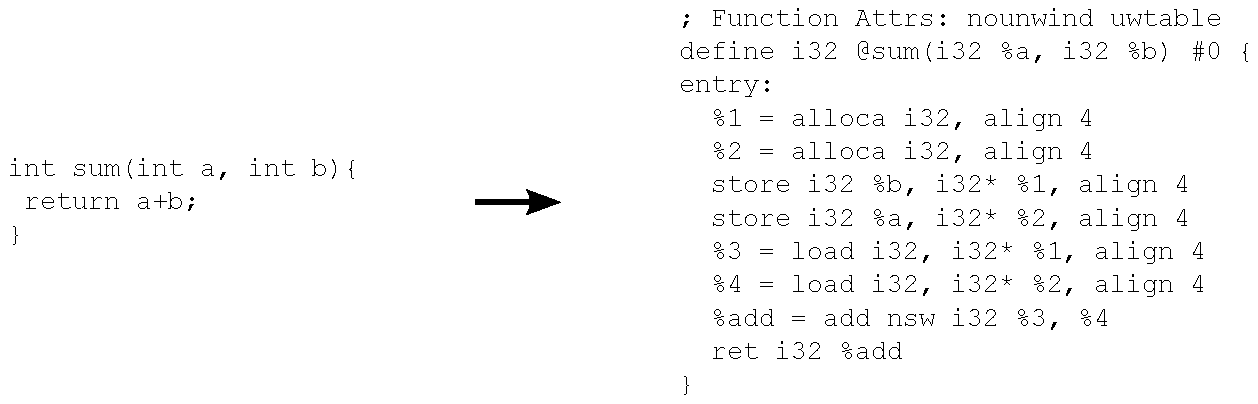
\includegraphics{fig/llvmir.pdf}}
    \caption{A C function and the {LLVM IR} equivalent}
    \label{fig_llvmir}
\end{figure}

\paragraph*{Module} The contents of a single {LLVM IR} file, be it binary bitcode or textual assembly form a module. A module is the top-level data structure in {LLVM IR}. The module contains information about target architecture, declarations of structured data types, declarations of external functions, global variables and a list of function definitions. The relationships between functions are apparent on this level and form a \emph{call graph}, in which nodes represent functions and an edge from $A$ to $B$ means that function $A$ calls function $B$ in its body.

\begin{figure}[H]
    \centering
    \scalebox{0.65}{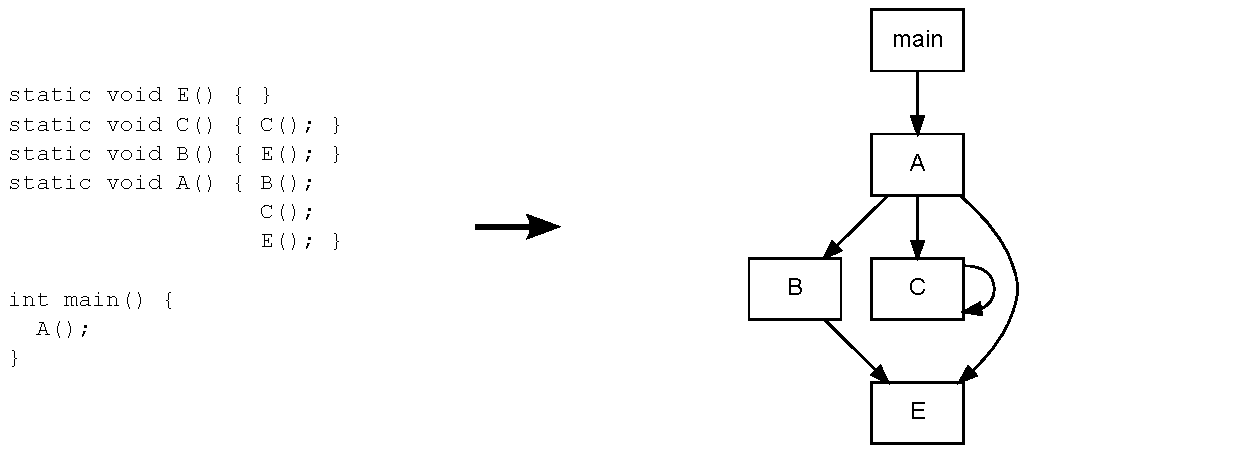
\includegraphics{fig/callgraph.pdf}}
    \caption{An example of a call graph}
    \label{fig_callgraph}
\end{figure}

\paragraph*{Function} Each function in {LLVM IR} has a list of formal arguments, a return type and a body consisting of basic blocks. Additionally it can have a number of optional attributes specifying a garbage collector, exception information, linkage type and so on. The first basic block in a function is denoted by the \texttt{entry} label. Local variables have a \texttt{\%} prefix while global variables have a \texttt{@} one. Relationships between basic blocks are apparent on this level and form a \emph{control flow graph}.

\paragraph*{Basic Block} A collection of IR instructions that is always executed sequentially. A basic block begins with a label that is used to reference the basic block in control flow instructions and ends with a terminator instruction, usually a \texttt{br} instruction which jumps to a label of another basic block or a \texttt{ret} instruction, which exits the function. Each basic block has a list of successors and predecessors in the control flow graph. In some cases the value of a variable in the basic block is dependent on the predecessor. To maintain SSA form a \emph{$\phi$-instruction} must be present in the basic block before the use of the variable.

\begin{figure}[H]
    \centering
    \scalebox{0.65}{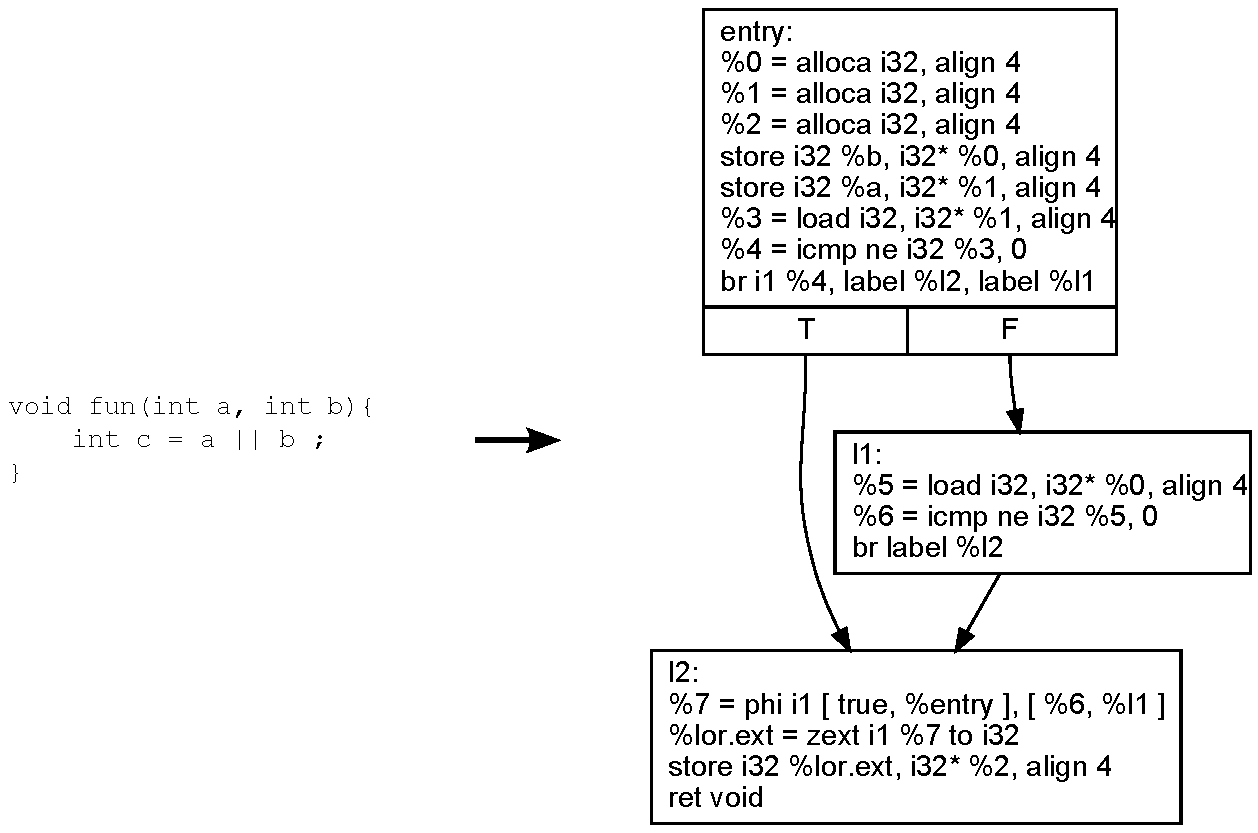
\includegraphics{fig/cfg.pdf}}
    \caption{Control flow graph with a $\phi$-instruction}
    \label{fig_cfg_phi}
\end{figure}

\chapter{Detector Implementation}
\label{ch_detector}
The general structure of a behavioral malware detector was introduced in chapter \ref{ch_malware}, section~\ref{s_behav_det}. This chapter introduces a proof-of-concept detector prototype which uses methods of formal analysis and verification. Since a robust and complete implementation of a behavioral malware detector exceeds the format of this work, simplifications with regard to the general detector scheme were made.

Most significantly static extraction has been replaced by an obfuscating compiler\cite{ollvm} capable of generating random mutations of malware written in C and C++. The output of the obfuscating compiler is an {LLVM IR} binary file which represents a raw characterictic in the general detector scheme. A set of mutations can be obtained by repeatedly running the compiler on the same malware source code.

Interpretation of the raw characteristics is done by static taint analysis, which can be formalized as an abstract interpretation. The goal of the analysis is to provide information about the analyzed malware which is used to form a behavioral signature. The signature needs to represent the malicious behavior precisely enough to minimize false negatives and abstract from other behavior to stay the same across mutations and not produce false positives on bening software. \emph{Syscall dependency graphs} were chosen for this purpose and correspond to the abstraction in the general detector scheme. Section \ref{s_abstractiob} covers details about dependency graphs and static taint analysis.

A set of dependency graphs is used to infer a classifier in the form of an automaton accepting a $k$-testable tree language. Since dependency graphs are general directed graphs, post-processing of the graphs needs to be done before inference. The matching phase of the general detector schema is done by checking whether an unknown dependency graph is accepted by an automaton inferred from dependency graphs of known malware. Post-processing of dependency graphs and inference algorithms are described in Section \ref{s_inference}.

\begin{figure}[H]
    \centering
    \scalebox{0.65}{
\includegraphics{todo.pdf}}
    \caption{Diagram of the implemented detector}
    \label{fig_detector}
\end{figure}

\section{Input Generation}
To reliably design a malware detector, representative inputs were needed. The first challenge when implementing the prototype was to find suitable malware source code. However malware is typically found in the form of binary files and source code is rare. Thankfully various internet community forums, such as \cite{rohitab}, provided examples of C and C++ code that exhibits typical malicious behavior. Three different keyloggers and two file infecting viruses were obtained. The complexity of the samples ranges from simple single-threaded code to multi-threaded code in which each thread is responsible for different malicious behavior.

\subsection{Obfuscator-{LLVM}} A modified {Clang/LLVM} compiler was used to generate mutations of the acquired malware samples. Obfuscator-{LLVM}, or \texttt{ollvm} for short, was built for the purpose of intellectual property protection, however its obfuscating transformations of {LLVM IR} can be well used for generating malware mutations. Four kinds of obfuscations are available in the public version of the compiler, one of which is instruction substitution which is covered in chapter~\ref{ch_malware}, section~\ref{s_polymorph}. The description of the other three follows.

\paragraph{Basic Block Splitting} As the name suggests, this transformation splits basic blocks at random locations and recovers original control flow by inserting unconditional branch instructions. The main purpose of this transformation is to amplify the effect of other obfuscations in \texttt{ollvm}.

\begin{figure}[H]
    \centering
    \scalebox{0.7}{
\includegraphics{todo.pdf}}
    \caption{Basic Block Splitting}
    \label{fig_bb_split}
\end{figure}

\paragraph{Control Flow Flattening} Designed for the purpose of making control flow analysis ineffective and expensive, the obfuscation transforms control flow inside a function to a flat structure using \texttt{switch-case} constructs. Original control flow is preserved using a control variable in a designated basic block.

\begin{figure}[H]
    \centering
    \scalebox{0.7}{
\includegraphics{todo.pdf}}
    \caption{Control Flow Flattening}
    \label{fig_flattening}
\end{figure}

\paragraph{Bogus Control Flow} An advanced form of dead code insertion which makes use of \emph{opaque predicates}. Extra basic blocks are insterted into the control flow of a function. These basic block contain a conditional jump to the original basic block and to a cloned version of it. However the jump is always made to the original basick block because the predicate always evaluates to the same value. The predicate is constructed in such a way that it is hard to evaluate statically. In figure \ref{fig_bcf} the original basic block \texttt{\%2} is cloned into \texttt{\%3} and preceded by \texttt{\%1} which contains the opaque predicate. The opaque predicate is $((x-1) \cdot x) \mod 2 = 0 \vee y \leq 10$ and always evaluates as true when $x$ and $y$ are integers. 

Futhermore some junk code is added into the original and the cloned basic block and inconsequential control flow from the cloned basic block is added. Finally one more opaque predicate is added to the original basic block, finishing a dead control flow loop. This will prove important in the following sections.

\begin{figure}[H]
    \centering
    \scalebox{0.65}{
\includegraphics{todo.pdf}}
    \caption{Bogus Control Flow}
    \label{fig_bcf}
\end{figure}

\section{Abstracting Behavior}
\label{s_abstraction}
%taint analysis and call dependency graphs, specifying taint sources and sinks in {LLVM IR}, taint analysis formalized as abstract interpretation, algorithm descriptions
After generating malware mutations the detector builds abstractions of their behavior in the form of \emph{syscall dependency graphs}, or SDGs for short. SDGs are directed graphs where nodes are calls to functions provided by the operating system and an edge from $A$ to $B$ tells that data computed from the result of a $A$ is used by $B$. Figure \ref{fig_sdg} shows an example of a malware SDG.

\begin{figure}[H]
    \centering
    \scalebox{0.65}{
\includegraphics{todo.pdf}}
    \caption{Syscall Dependency Graph}
    \label{fig_sdg}
\end{figure}

The reason why SDGs were chosen is because they abstract from all of the internal computations of the malware, where most obfuscations happen, and focus only on how the malware interacts with its host system. Although certain aspects of the interaction can change between mutations, e.g., the order in which the syscalls are made, the dependecies between them generally do not change. To get the information needed to build an SDG, static taint analysis is performed.

\subsection{Static Taint Analysis}
The idea behind static taint analysis is to mark the data we wish to track as tainted, mark the origins of tainted data as \emph{taint sources} and mark points beyond which we do not track tainted data as \emph{taint sinks}. Taints then flow through the code according to predefined \emph{propagation rules}. A formalization of this concepts is given in Definition \ref{def_taint} and the implemented algorithm is described in Algorithm \ref{alg_taint}.

\begin{defn}
\label{def_taint}
Let \texttt{Var} be set of program variables, \texttt{Instr} an instruction set, \texttt{Src} $\subseteq$ \texttt{Instr} a set of taint sources and \texttt{Snk} $\subseteq$ \texttt{Instr} a set of taint sinks. \emph{Static taint analysis} is an abstract interpretation $$I = (Q, \circ, \sqsubseteq, \bot, \top, \tau)$$ where
    \begin{itemize}
        \item $Q$ is a set of mappings of the form $C: \text{\texttt{Var}} \rightarrow 2^T$,
        \item $\circ: Q \times Q \rightarrow Q$ is a join operator such that $\forall a \in \text{\texttt{Var}}: (C_1 \circ C_2)(a) = C_1(a) \cup C_2(a)$,
        \item $(\sqsubseteq) \subseteq Q \times Q$ is a partial order such that $C_1 \sqsubseteq C_2 \Longleftrightarrow \forall a \in \text{\texttt{Var}}: C_1(a) \subseteq C_2(a)$,  
        \item $\bot$ is a mapping $C$ such that $\forall a \in \text{\texttt{Var}}: C(a) = \emptyset$,
        \item $\top$ is a mapping $C$ such that $\forall a \in \text{\texttt{Var}}: C(a) = T$,
        \item $\tau: \text{\texttt{Instr}}\times Q \rightarrow Q$ is an interpretation of abstract transformers such that
        \begin{equation*}
            \forall \text{\texttt{I}} \in \text{\texttt{Instr}}, \; \forall C \in Q: \tau(\text{\texttt{I}},C) = 
            \begin{cases}
                Create(\text{\texttt{I}}, C) & \text{ if \texttt{I}} \in \text{\texttt{Src}}\\
                Sink(\text{\texttt{I}}, C) & \text{ if \texttt{I}} \in \text{\texttt{Snk}}\\
                Propagate(\text{\texttt{I}}, C) & \text{ otherwise}
            \end{cases}
        \end{equation*}
    \end{itemize}
For an abstract context $C$ and an instruction \texttt{I}:
\begin{itemize}
    \item $Propagate(\text{\texttt{I}}, C)$ taints outputs of \texttt{I} by the union of taints carried by inputs of \texttt{I},
    \item $Create(\text{\texttt{I}}, C)$ uses $Propagate(\text{\texttt{I}}, C)$ and additionally taints outputs of \texttt{I} by \texttt{I},
    \item $Sink(\text{\texttt{I}}, C)$ sets all taints carried by inputs of \texttt{I} to $\emptyset$.
\end{itemize}
\end{defn}

\begin{algorithm}[H]
    \begin{algorithmic}
        \State{\textbf{Input:} Function F in {LLVM IR};}
        \State{\textbf{Output:} Abstract Context $C_n$ such that $C_{n-1} = C_n$;}
        \State{}
        \State$Q_{K} := \{s_{K}\}; \; \Sigma_{K} := \Sigma_{T}; \; R_{K} := \{\}; \; F_{K} := \{\}; \; A~:= \{\}; \; B := \{\}; \; C := \{\}; \; D := \{\}$;
    \end{algorithmic}
    \caption{Static taint analysis algorithm over an {LLVM IR} function}
    \label{alg_taint}
\end{algorithm}

In the detector implementation, taint sinks and taint sources coincide and are represented by {LLVM IR} call instructions which call a function that is tagged with \texttt{dllimport}. While the tag isn't tailored to this purpose, it is a good and easy approximation. A precise solution would require an enumeration of all the functions that the operating system provides.

\section{Classifier Inference}
\ref{s_inference}
graph post-processing (dir. cyc. graph -> DAG -> Tree), brief desc. of TA inference implementation
\section{Testing and Results}
test set, detection threshold, results
\chapter{Conclusion}
\label{ch_conclusion}
what was the work about, interpreting results, goals vs results
\section{Discussion}
taint analysis alterantives, alternative post-processing, alternative inference algos
\section{Future Work}
pointer analysis, smt solvers as a solution to opaque predicates, more accurate description of winapi calls as taint sources and sinks

%=========================================================================
